\begin{figure}
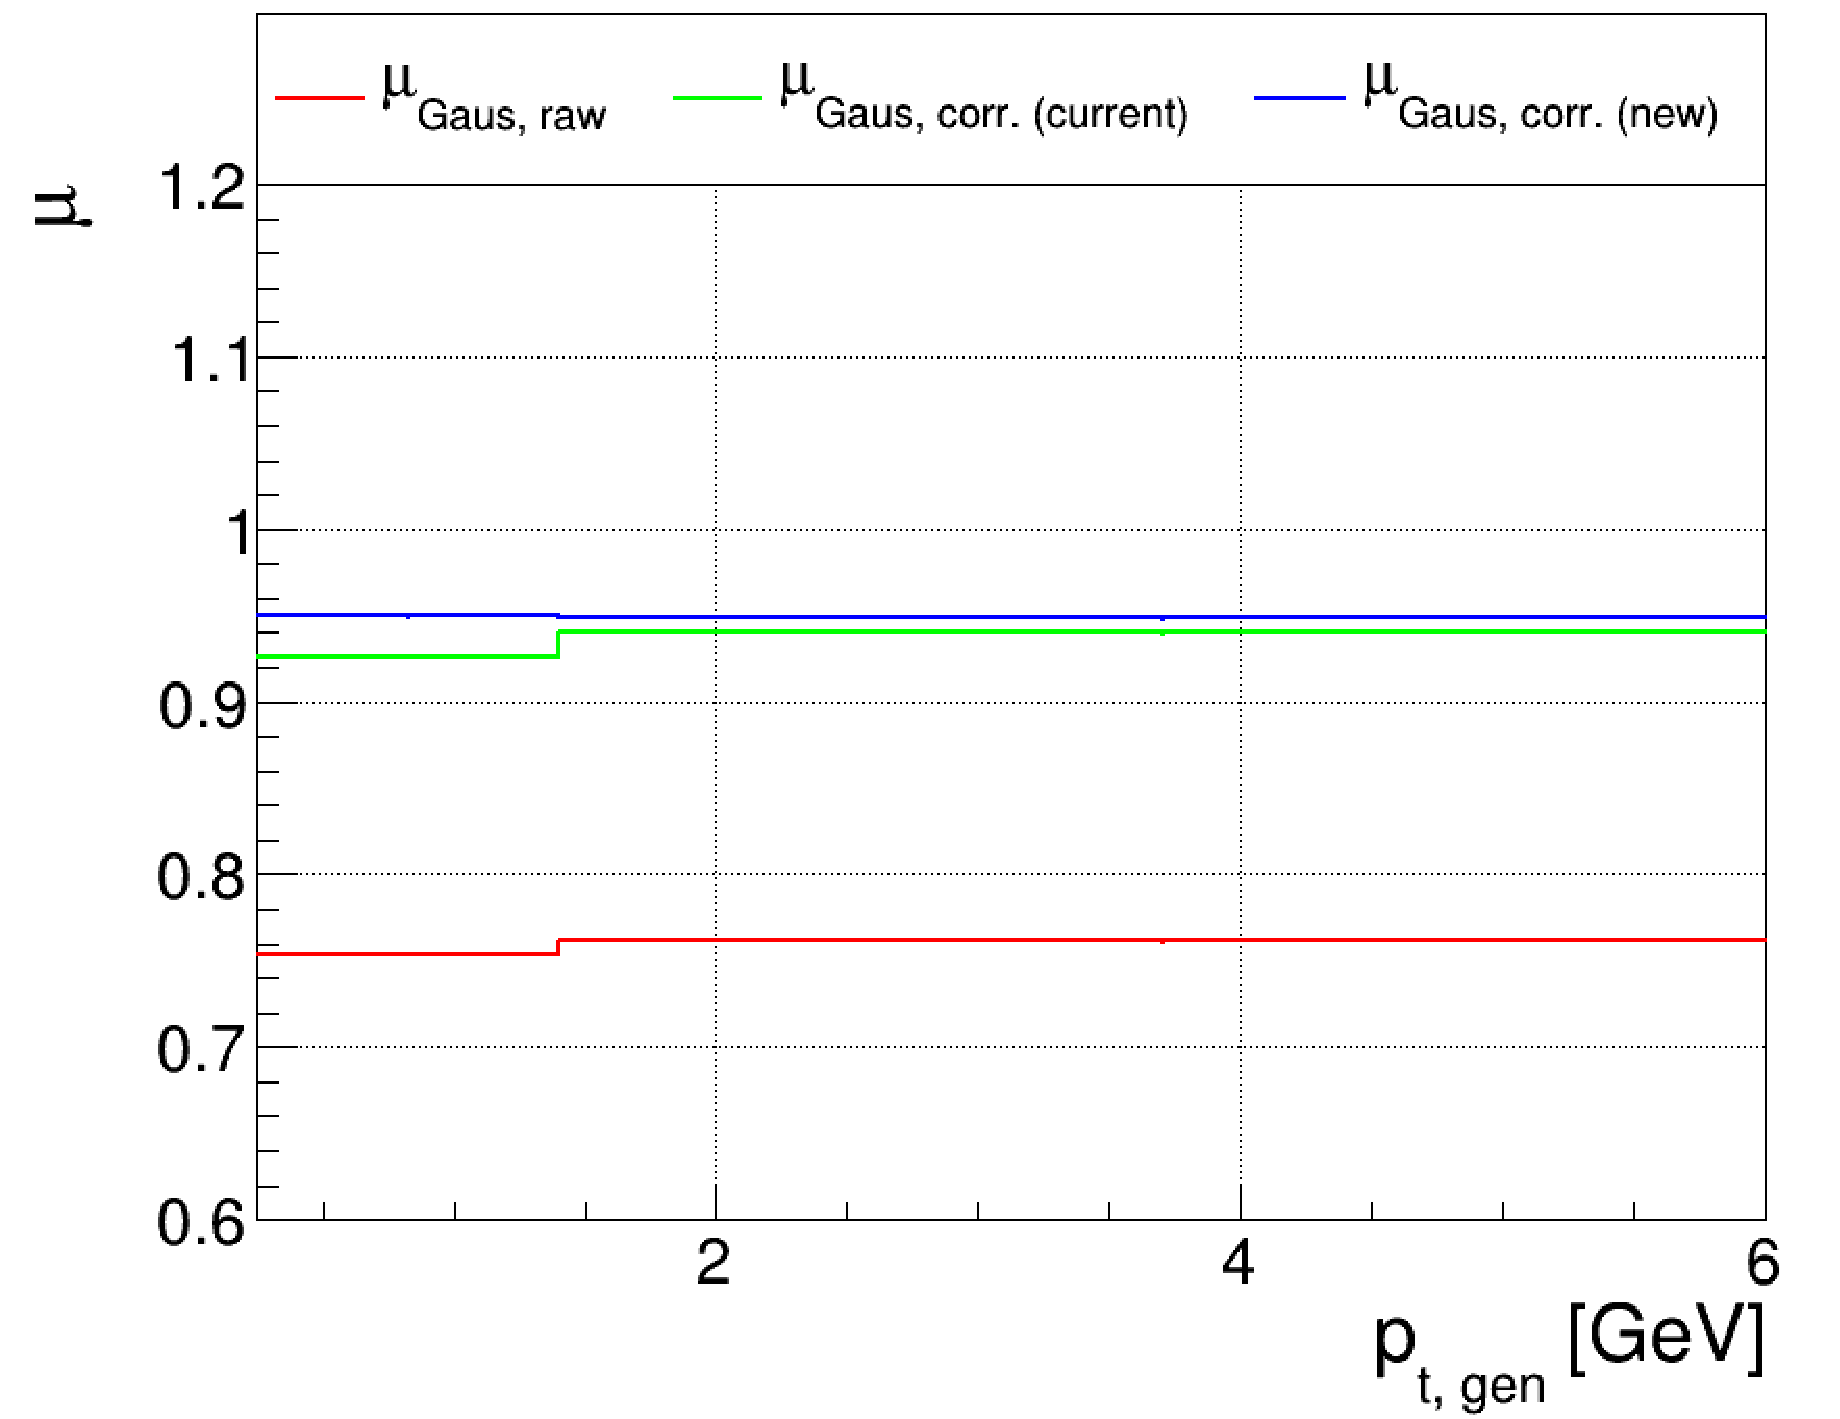
\includegraphics[width=0.495\textwidth]{./plots_pdf/ECAL_plots/plotsPU/EB/ZS/pdf/GENPT/EBZS_GENPT_0000_0006_MuOverBins.pdf}
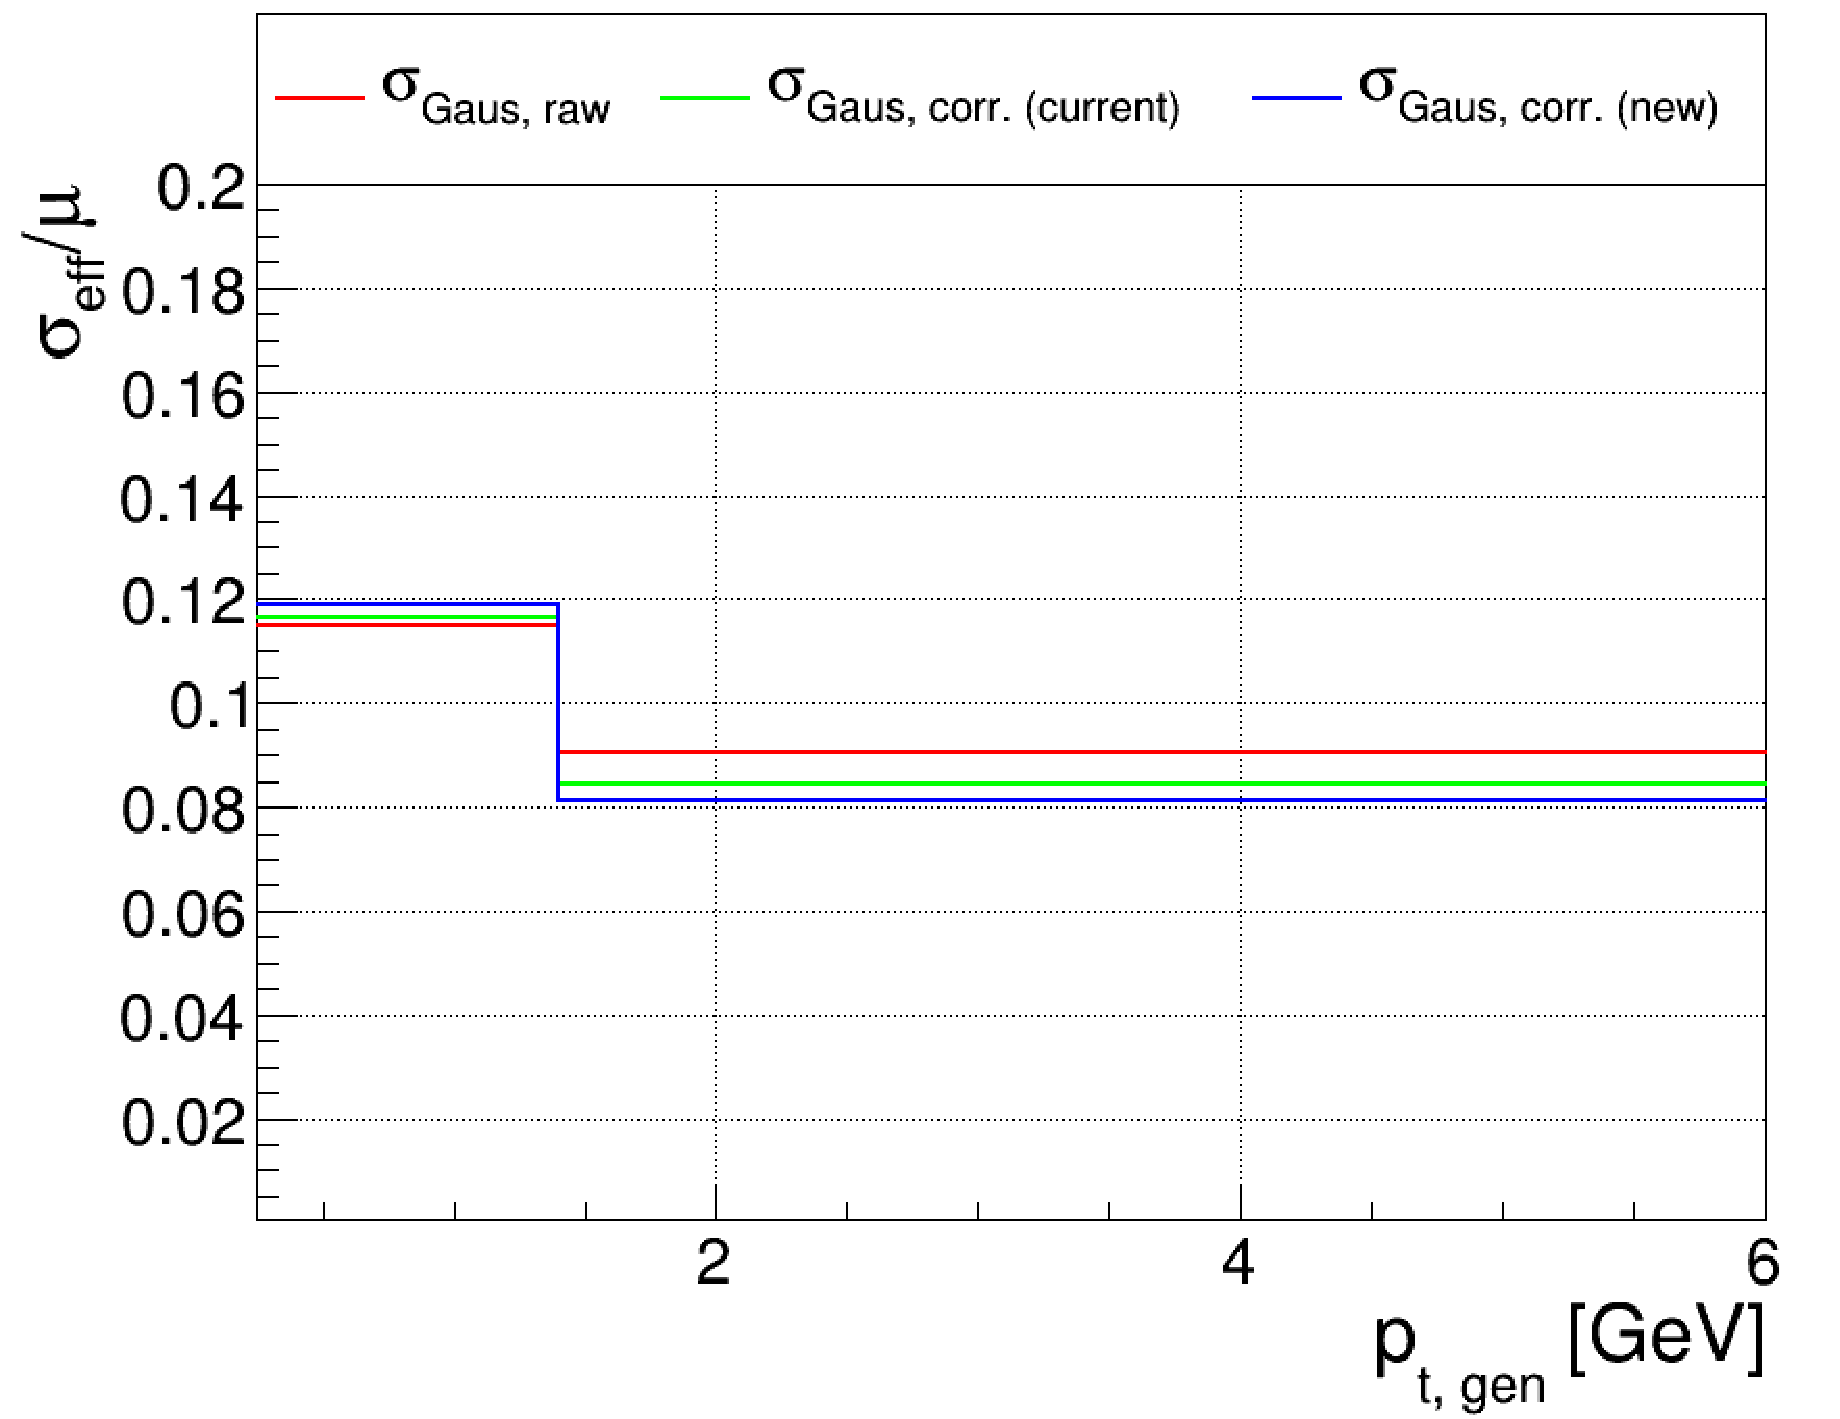
\includegraphics[width=0.495\textwidth]{./plots_pdf/ECAL_plots/plotsPU/EB/ZS/pdf/GENPT/EBZS_GENPT_0000_0006_EffSigmaOverBins.pdf}

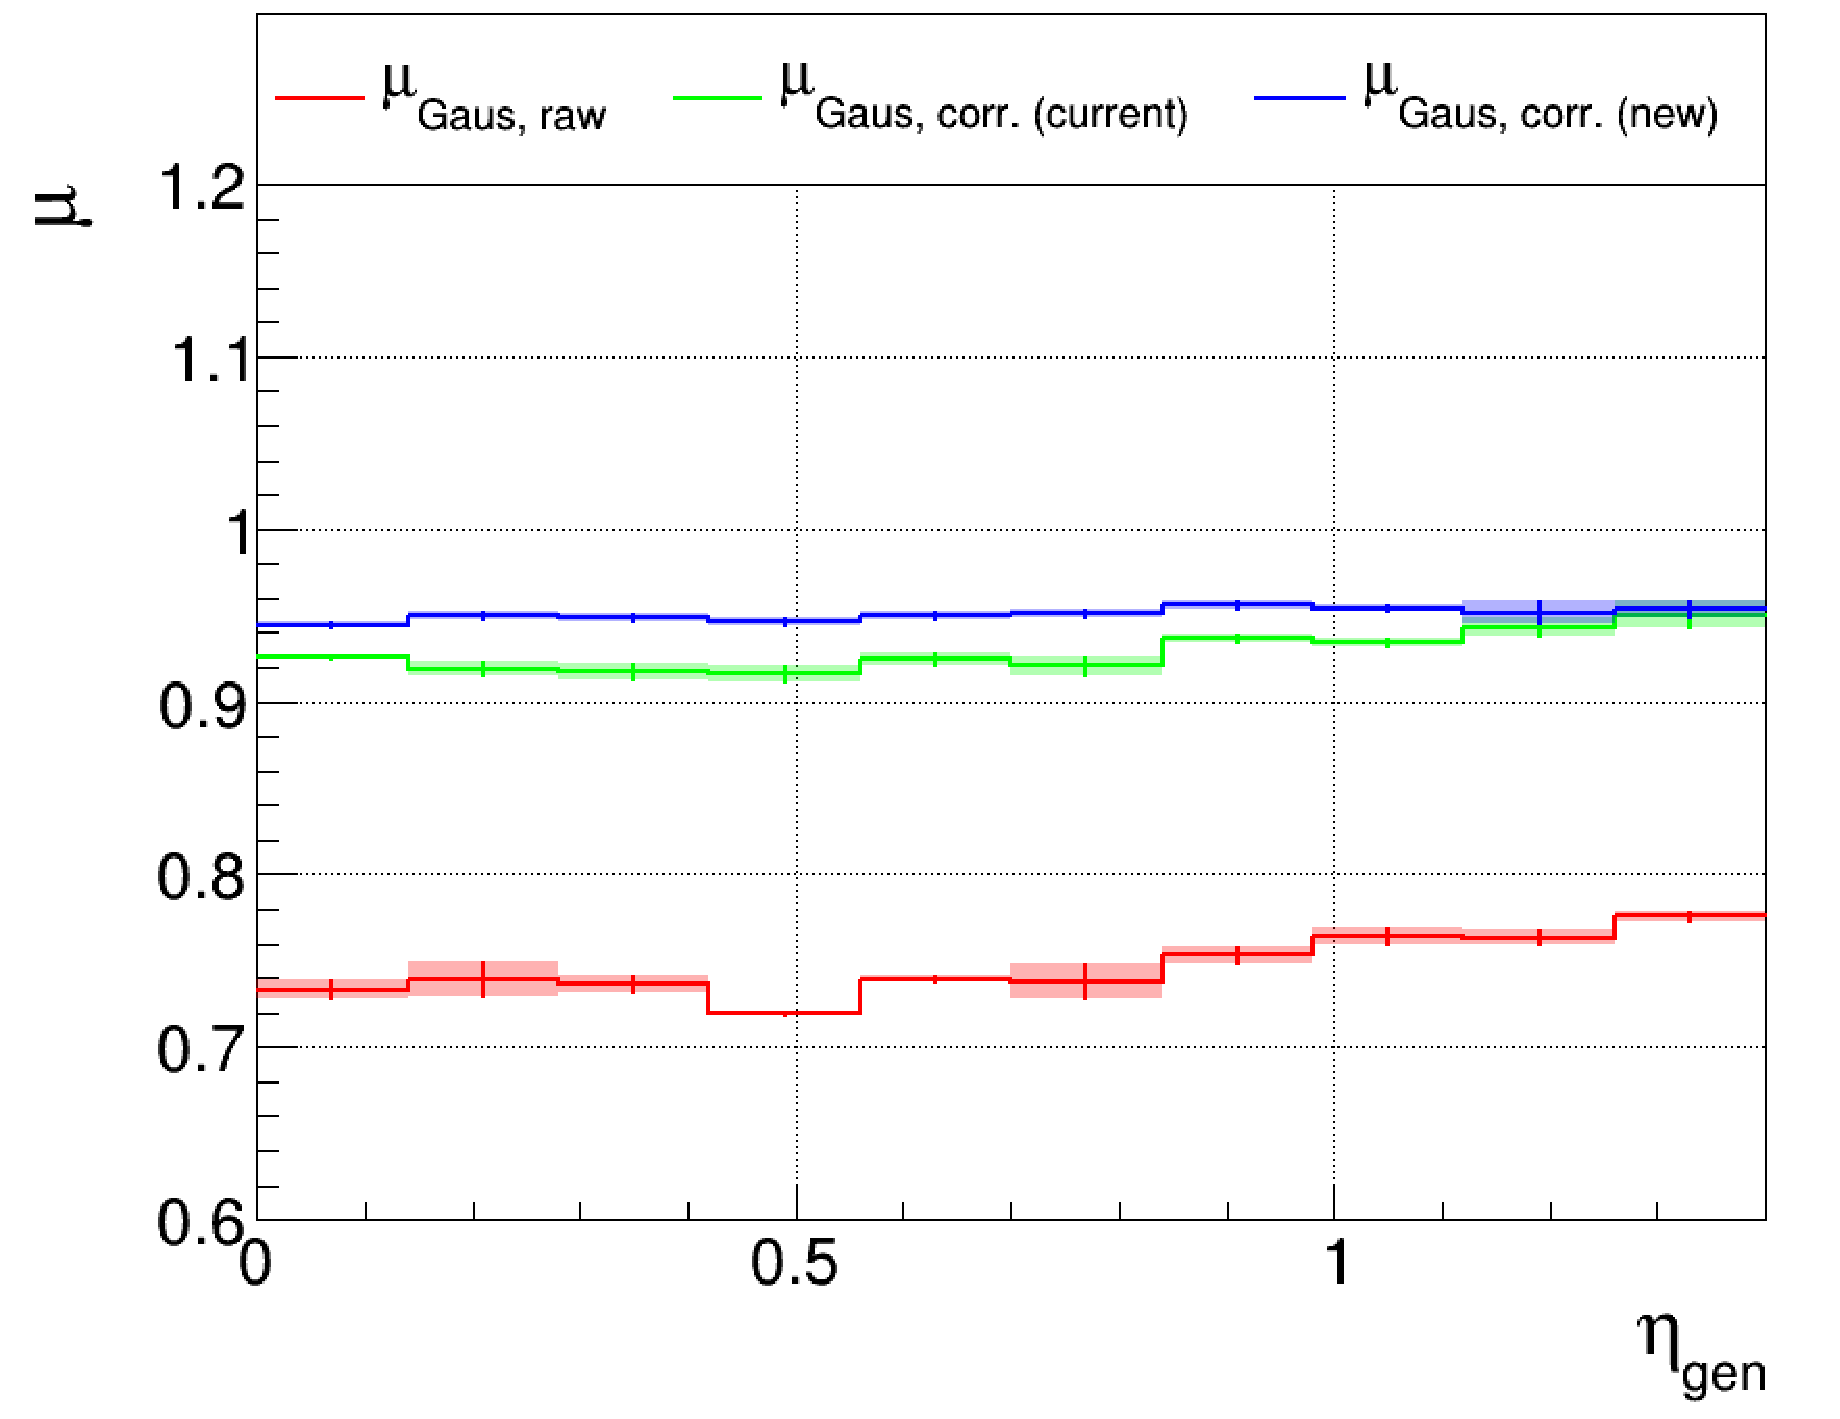
\includegraphics[width=0.495\textwidth]{./plots_pdf/ECAL_plots/plotsPU/EB/ZS/pdf/GENETA/EBZS_GENETA_0000_0006_MuOverBins.pdf}
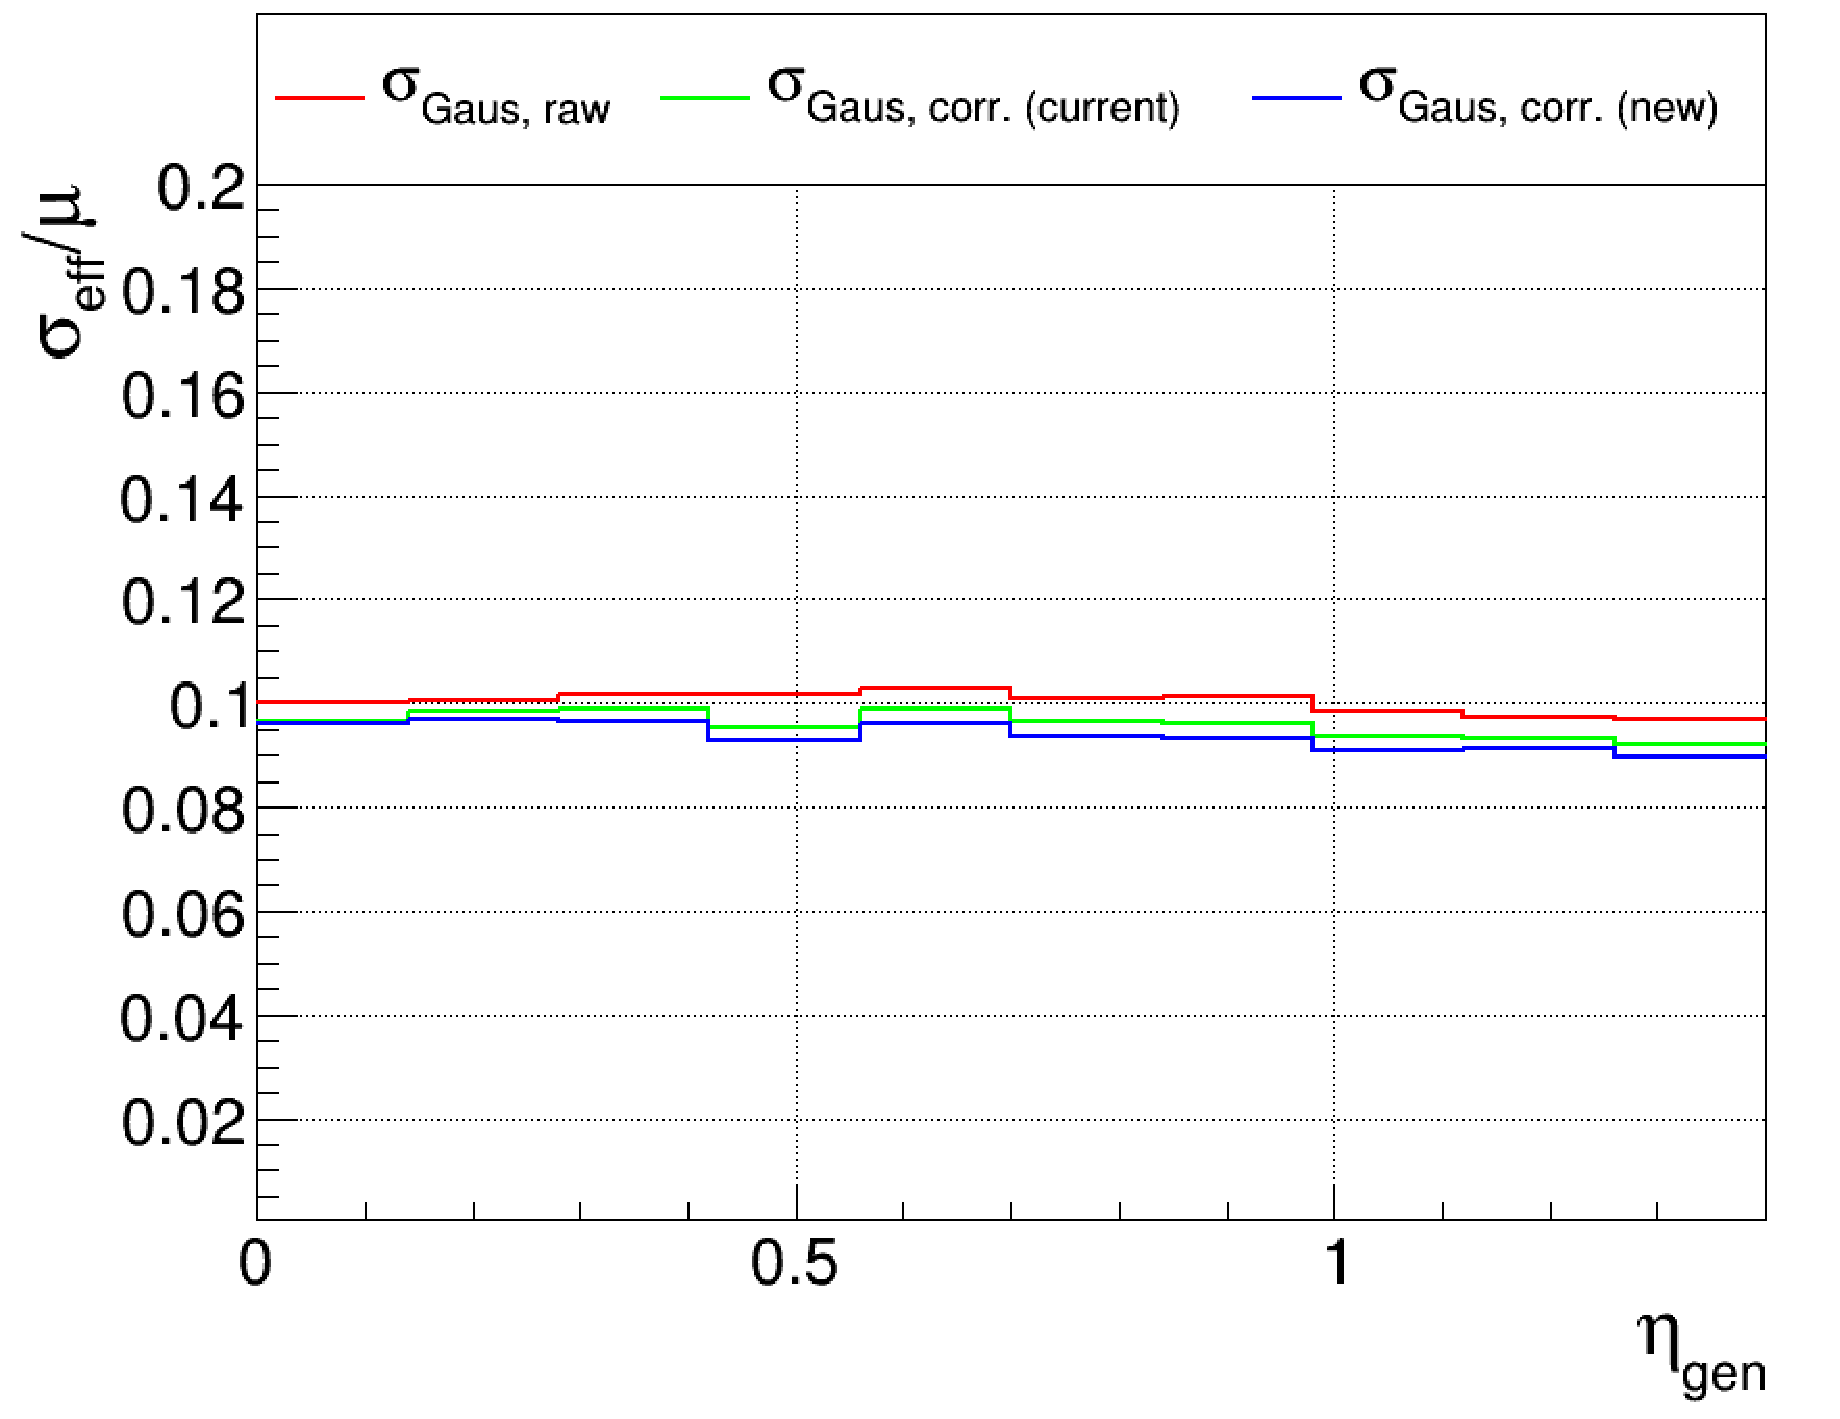
\includegraphics[width=0.495\textwidth]{./plots_pdf/ECAL_plots/plotsPU/EB/ZS/pdf/GENETA/EBZS_GENETA_0000_0006_EffSigmaOverBins.pdf}
\caption[$\mu$ ($\sigma_\mathrm{eff}$) vs \pt of PF ECAL cluster - EB ZS readout PU  senario]{Mean response (resolution) defined by Raw PF ECAL clusters (red), the calibration derived earlier in Ru\
n3 based on 126X (green), and the new correction from 2024 simulation sample based on 133X (blue). \pt 0--6\GeV PU EB ZS readout PU senario.}
\label{fig:PU_EBZS}
\end{figure}

%% %\begin{figure}
%% 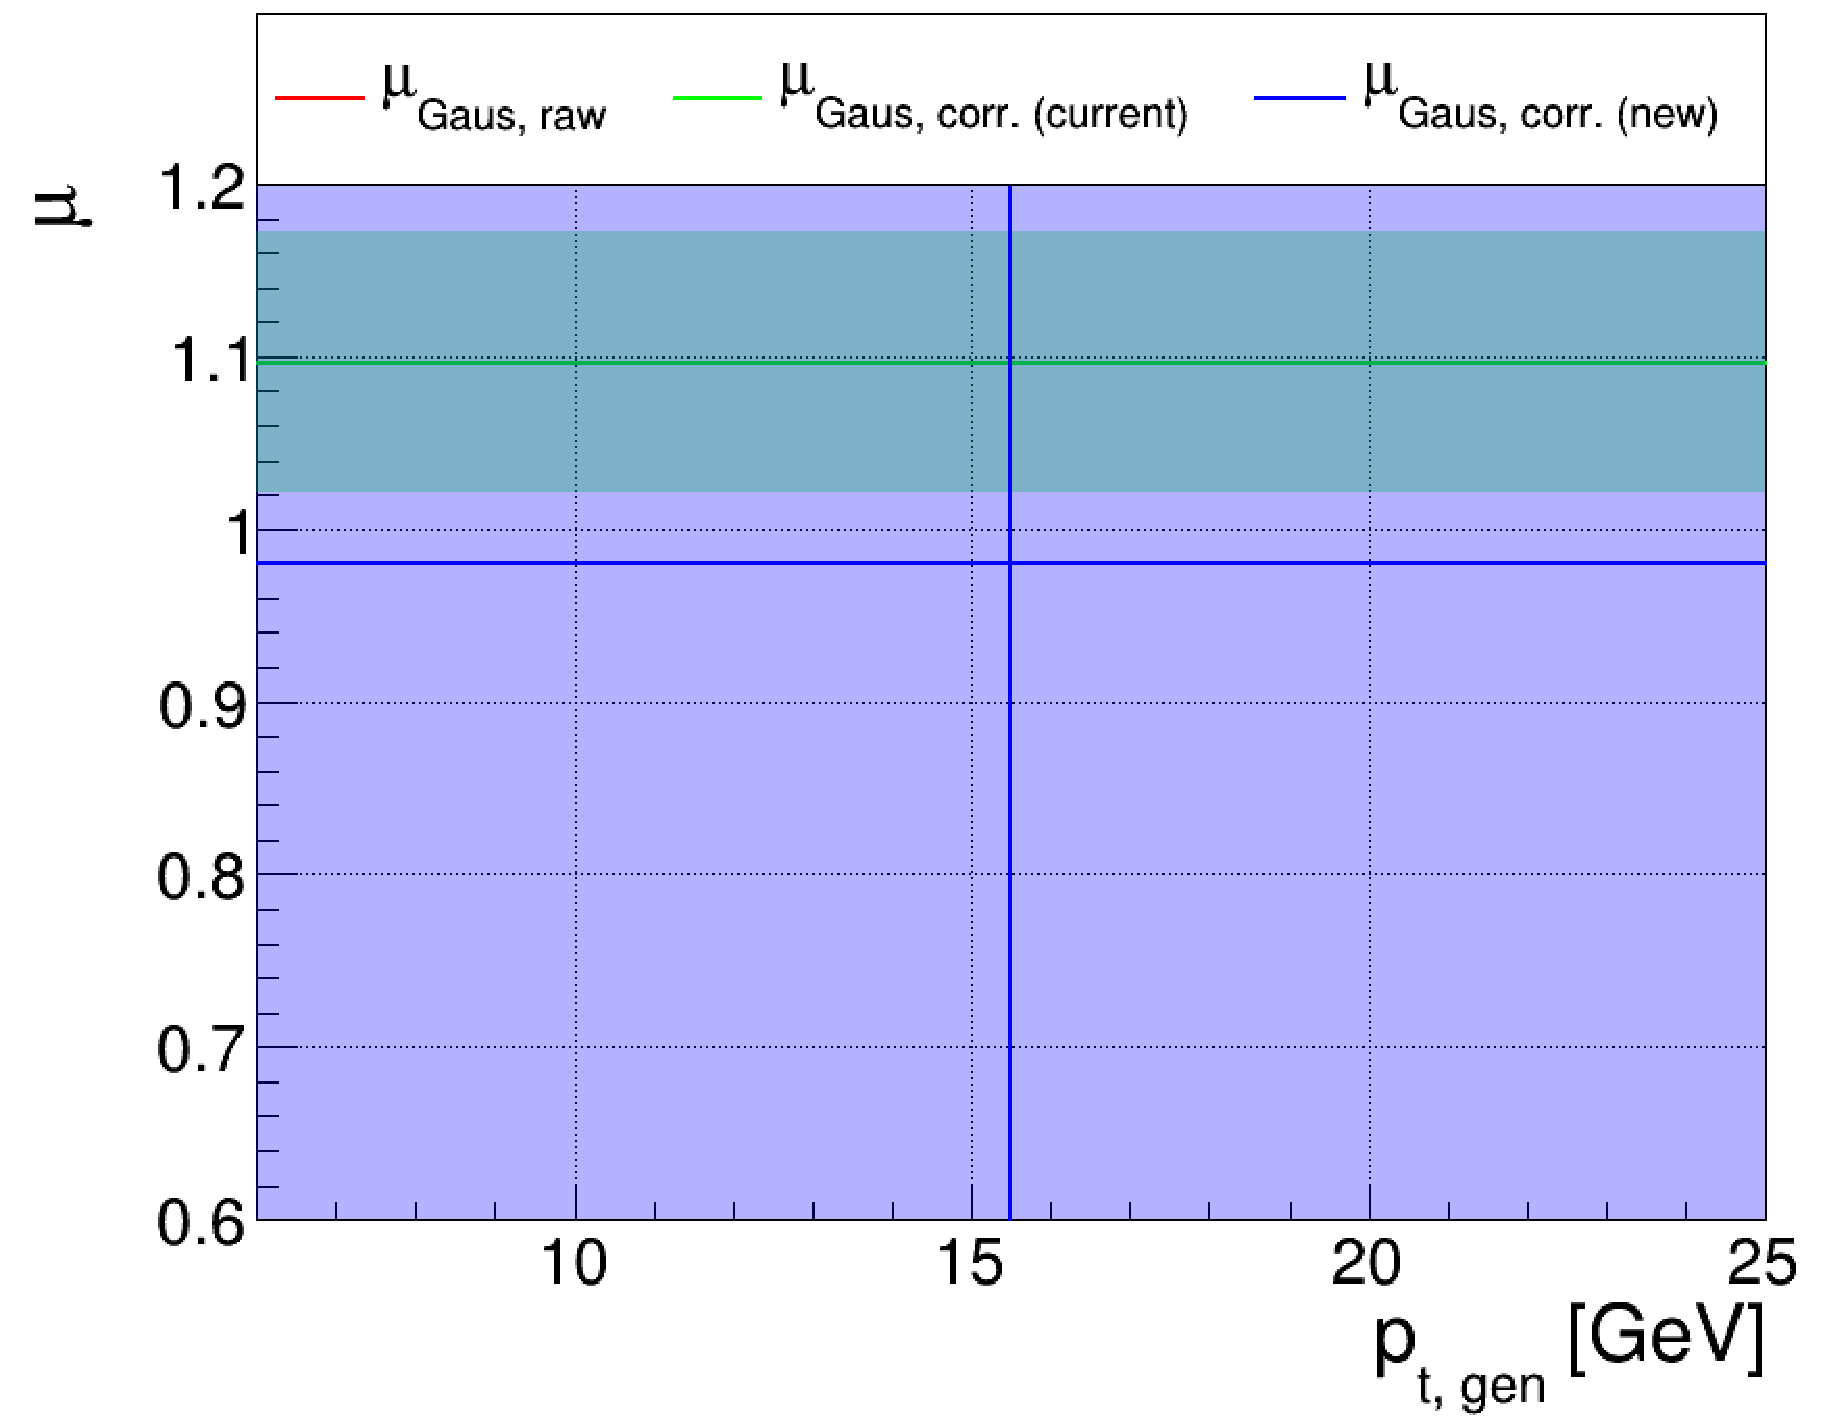
\includegraphics[width=0.495\textwidth]{./plots_pdf/ECAL_plots/plotsPU/EB/ZS/pdf/GENPT/EBZS_GENPT_0006_0025_MuOverBins.pdf}
%% 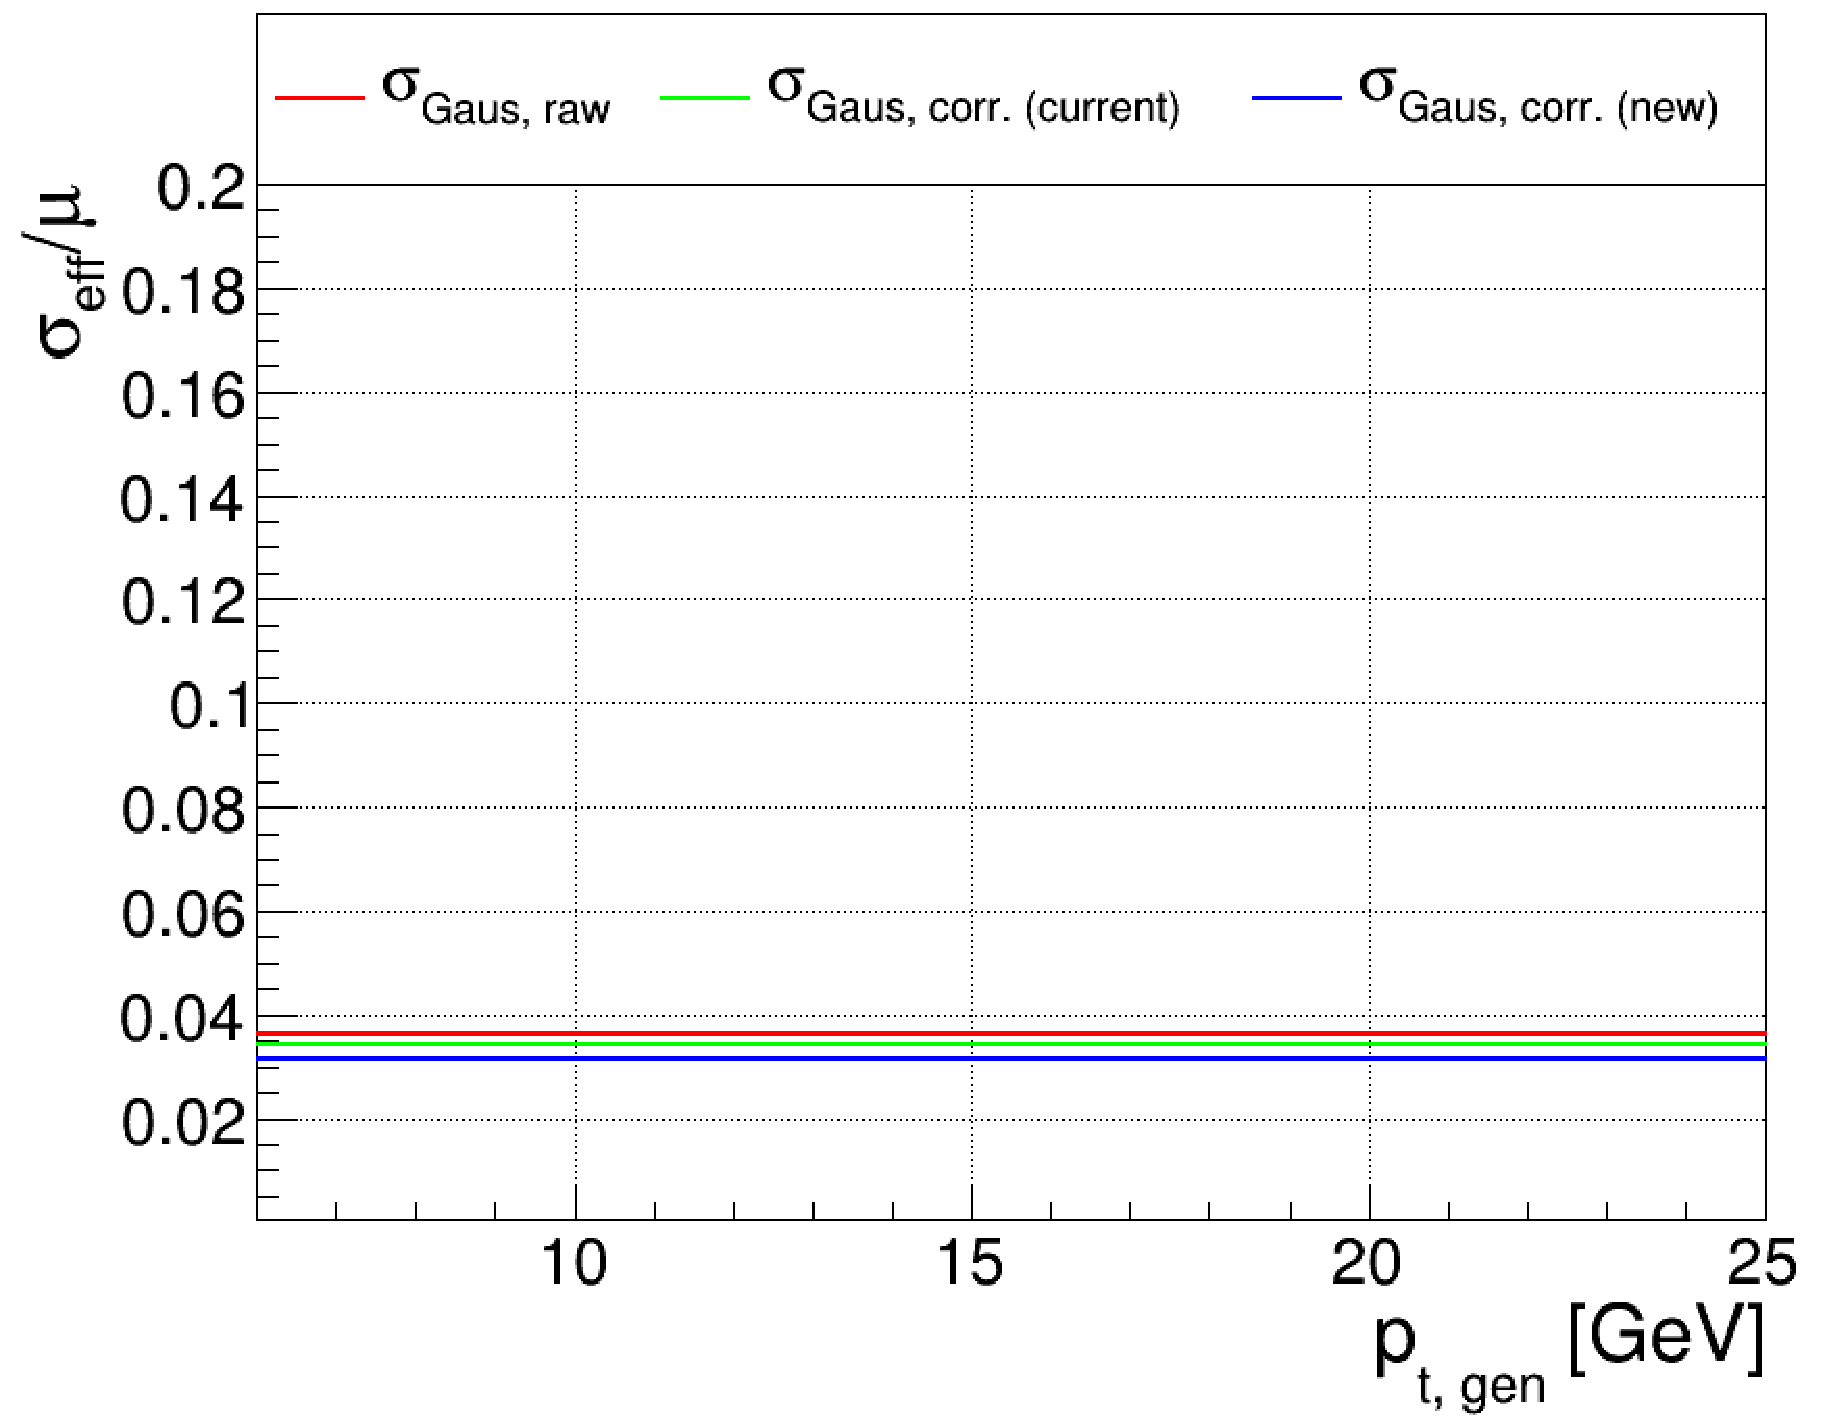
\includegraphics[width=0.495\textwidth]{./plots_pdf/ECAL_plots/plotsPU/EB/ZS/pdf/GENPT/EBZS_GENPT_0006_0025_EffSigmaOverBins.pdf}
%% %\caption{EB - ZS Readout pt 6-25}
%% %\end{figure}
%% %\begin{figure}
%% 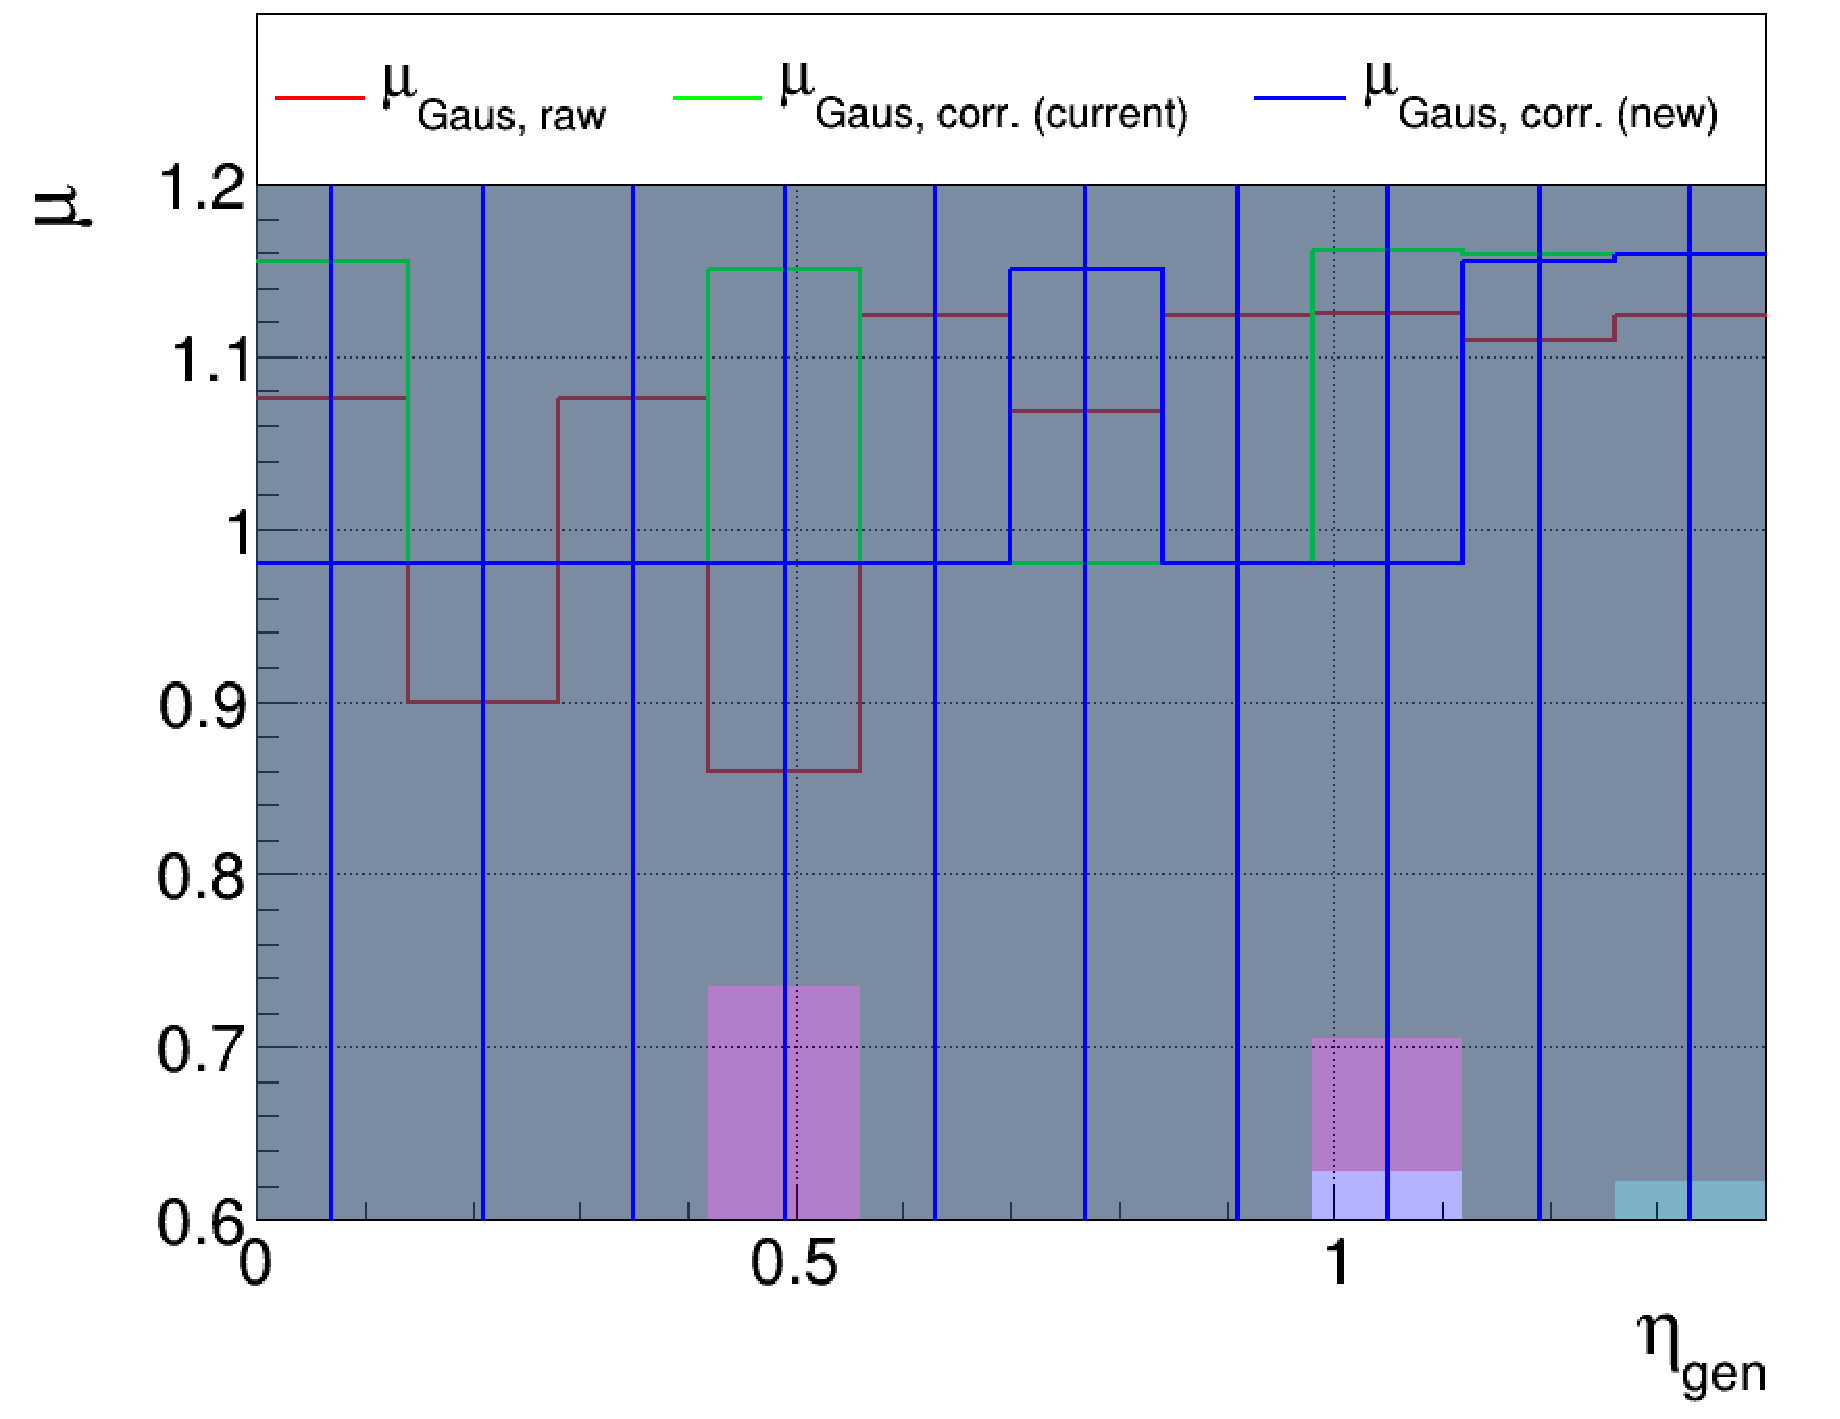
\includegraphics[width=0.495\textwidth]{./plots_pdf/ECAL_plots/plotsPU/EB/ZS/pdf/GENETA/EBZS_GENETA_0006_0025_MuOverBins.pdf}
%% 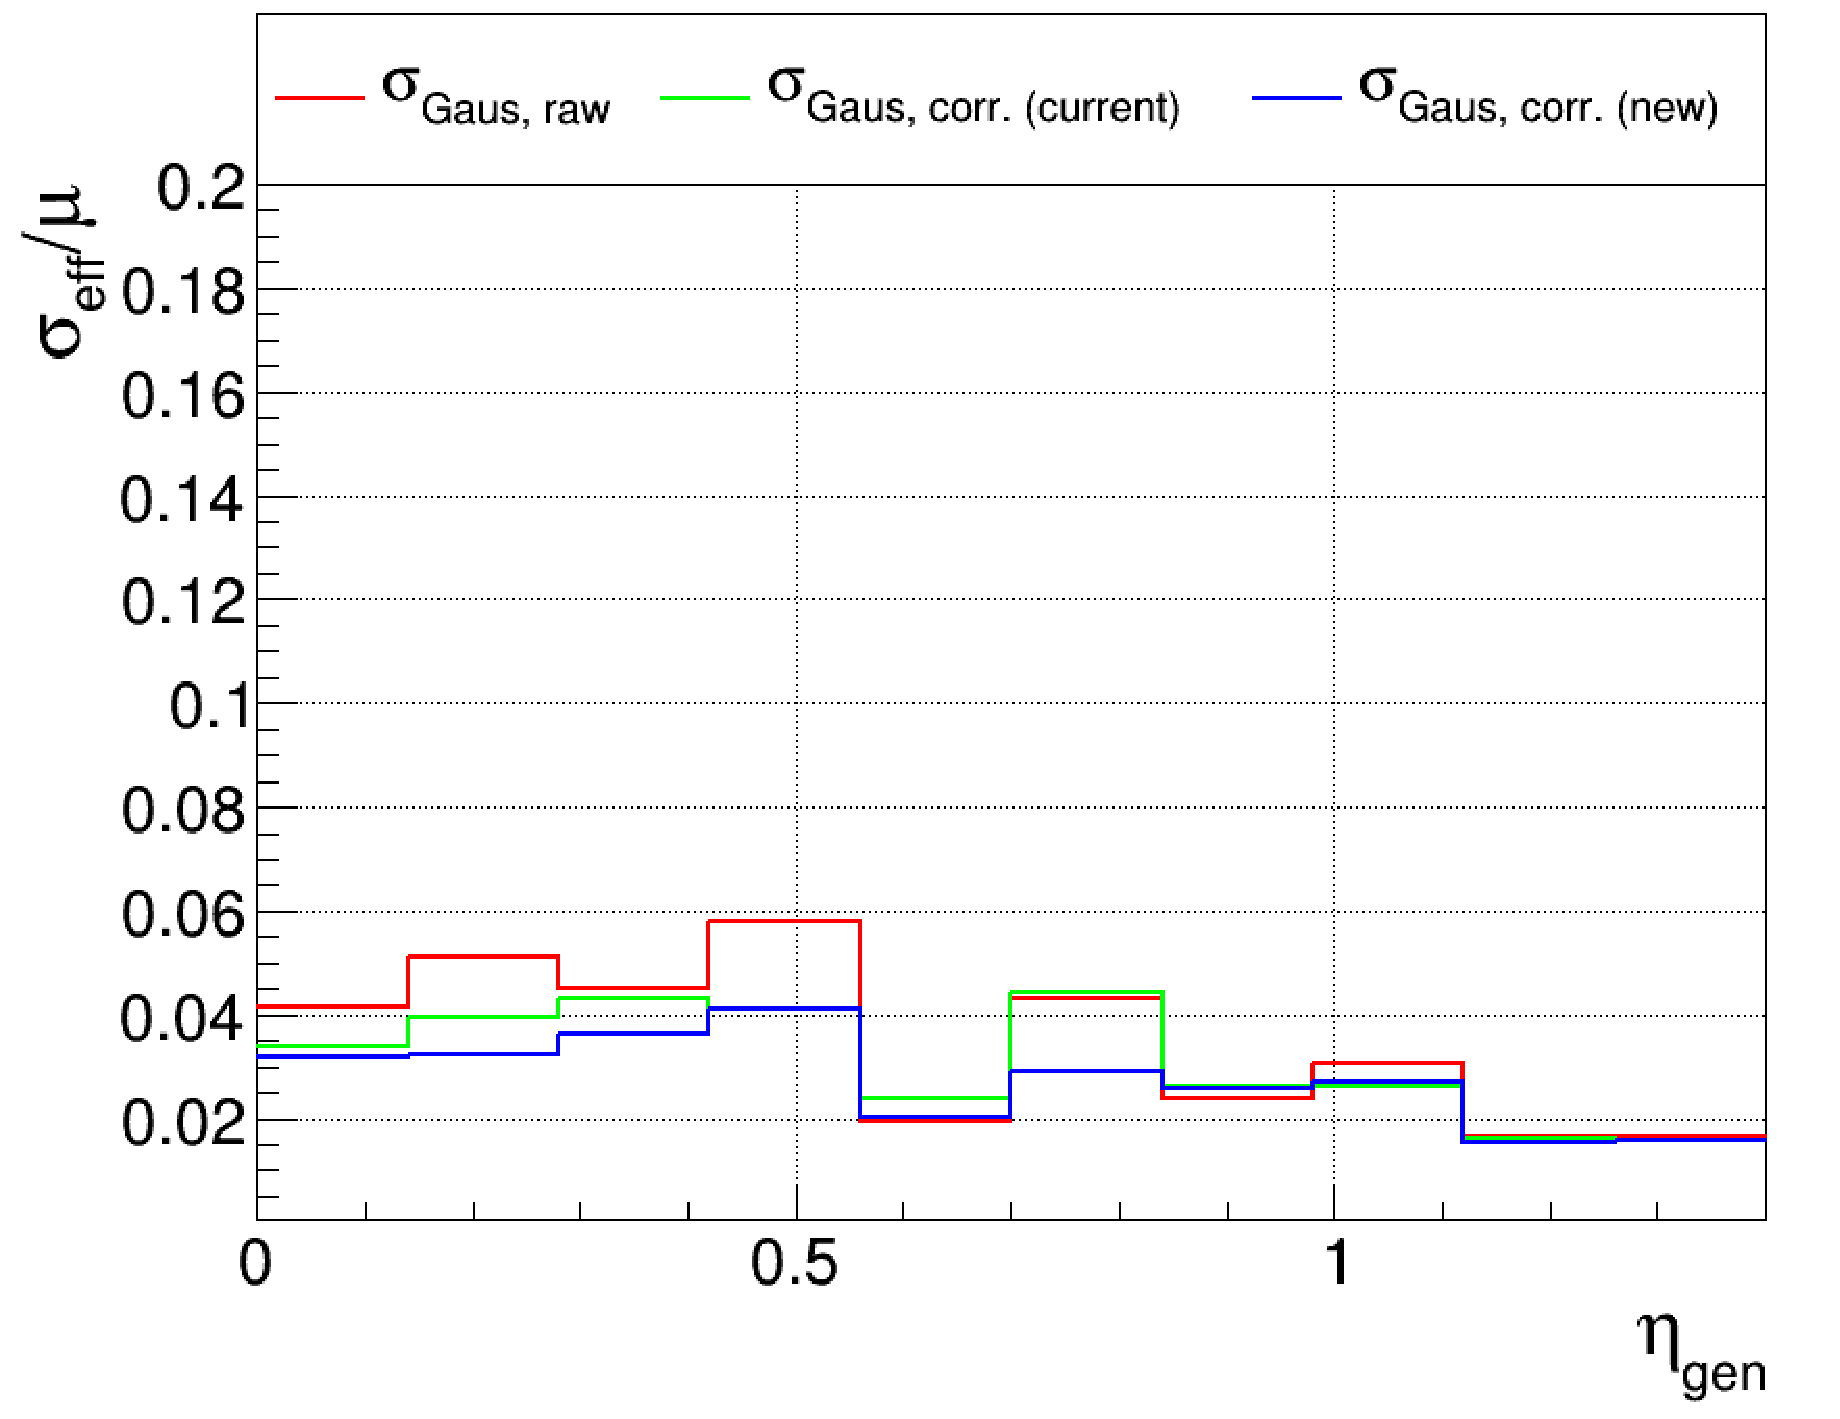
\includegraphics[width=0.495\textwidth]{./plots_pdf/ECAL_plots/plotsPU/EB/ZS/pdf/GENETA/EBZS_GENETA_0006_0025_EffSigmaOverBins.pdf}
%% \caption{EB - ZS Readout \pt 6-25}
%% \end{figure}





